\section{Ensemble Methods}
\begin{minipage}{0,5\linewidth}
	Instead of expecting a single model to perform best on all data, we train multiple models and aggregate their results. Techniques: Bagging, Pasting. 
\end{minipage}
\begin{minipage}{0,5\linewidth}
	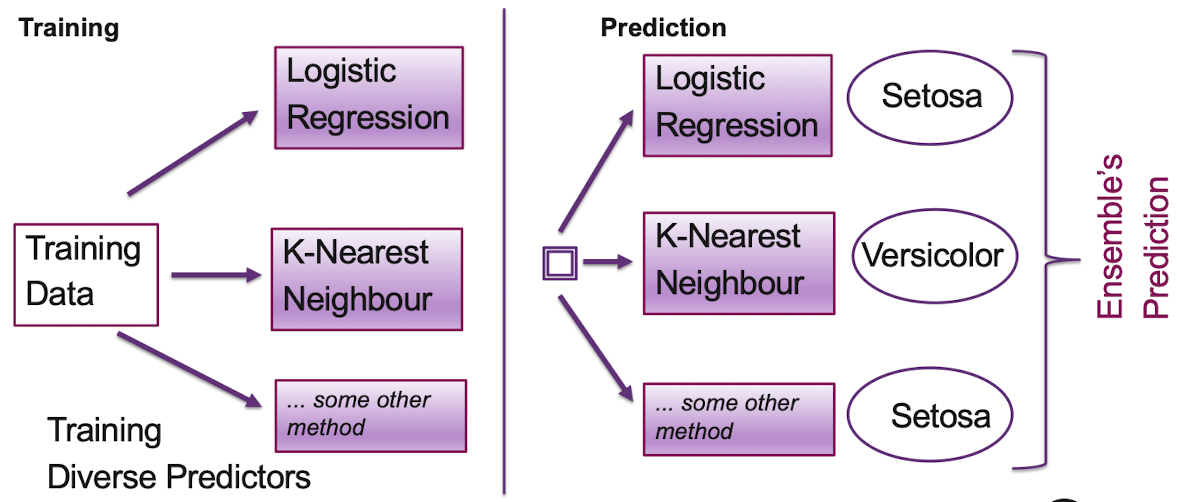
\includegraphics[width=\linewidth]{ensemble}  
\end{minipage}

\subsection{Dimensions}
We can use multiple methods for the classification of our data. These different methods can then be combined. Different learners use different algorithms, hyperparameters and training data. Additionally we can also apply the Cross Validation Pattern.

\subsection{Voting}
We can aggregate the predictions of weak learners with either soft or hard voting.\\
\textbf{Hard Voting:} Predict the class that gets the most votes, \textbf{Softvoting:} Predict the class with the highest class probability, averaged over all classifiers.
 
\subsection{Bagging and Pasting}
\textbf{sampling with replacement (Bagging)}: a data point can be selected more than once, \textbf{sampling without replacement (Pasting): a data point can be selected only once}.

\subsubsection{Out of Bag evaluation}
 In Bagging, some data points may be used several times. 

\subsection{No free lunch theorem}
no single machine learning algorithm is universally the best-performing algorithm for all problems". Evaluations! Since a predictor never sees out-of-bag (oob) data, it can be evaluated on oob data. No need for a separate validation or cross-validation set.